\documentclass[20pt,a4paper,landscape]{extarticle}
\usepackage[margin=1.45cm,top=0.45cm,left=0.9cm,right=0.9cm,bottom=0.9cm]{geometry}
\usepackage{amsmath}
\usepackage{amssymb}
\usepackage{graphicx}
\usepackage{xcolor}
\usepackage[sfdefault,lf]{FiraSans}
\renewcommand{\familydefault}{\sfdefault}
\setlength{\parindent}{0pt}
\pagestyle{empty}
\everymath{\displaystyle}
\begin{document}
\sffamily
\boldmath
{\LARGE \textbf{Estimating lengths from scale drawings and photos --- Excellence}}\par\vspace{0.45em}
\begin{center}
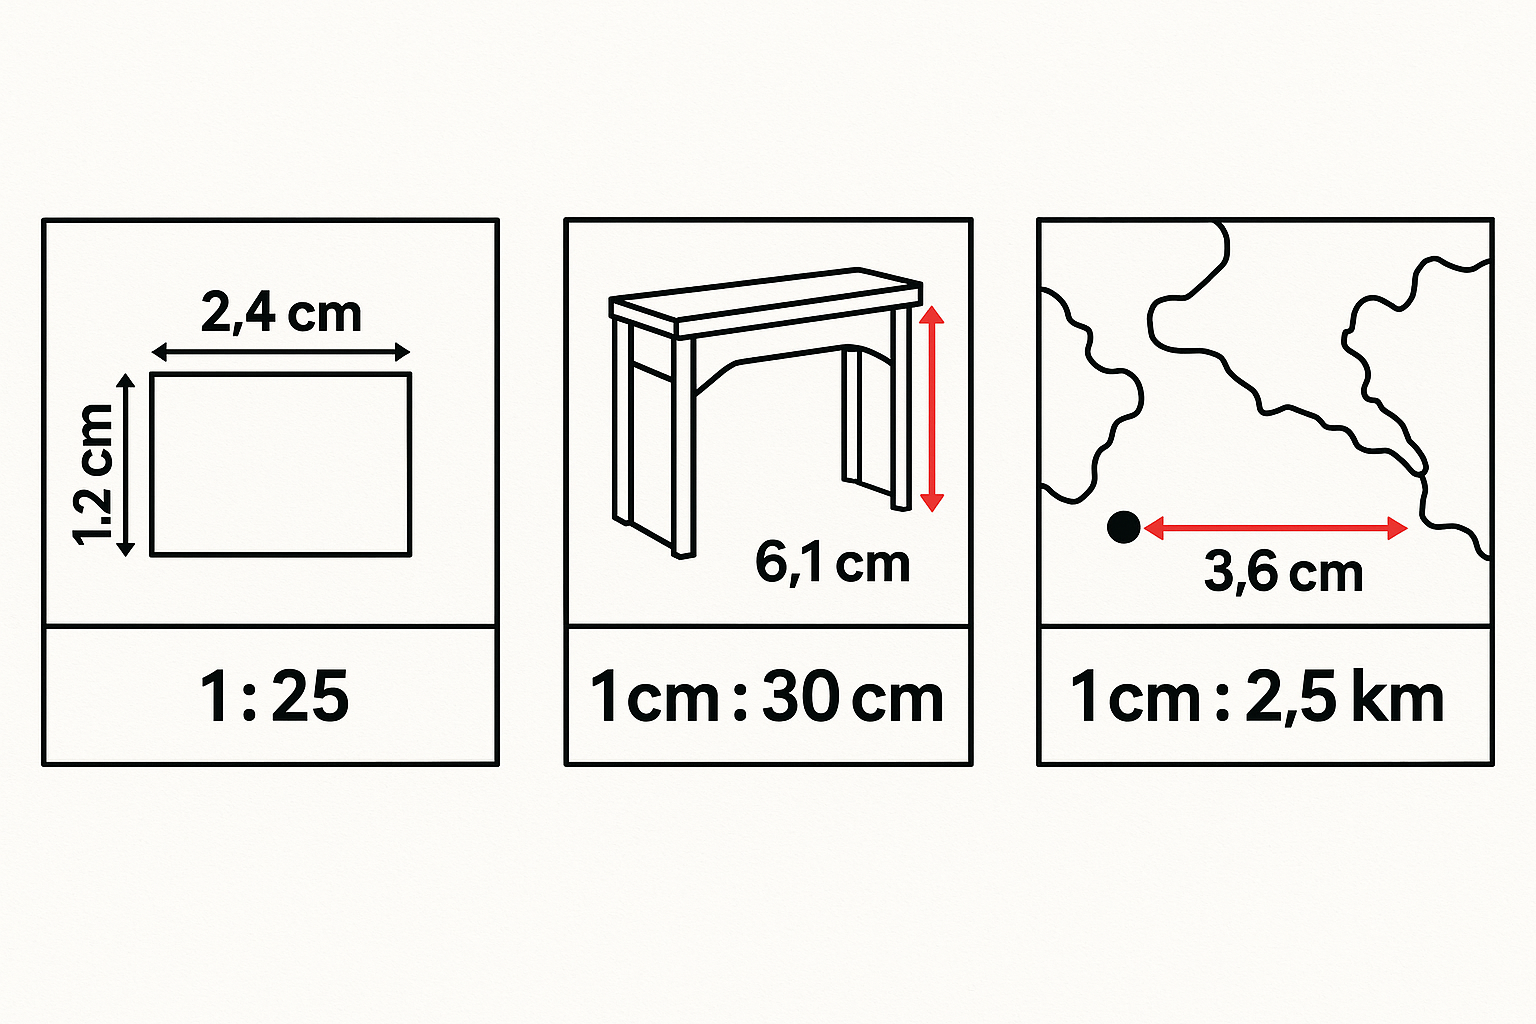
\includegraphics[width=0.94\linewidth,height=0.49\textheight,keepaspectratio]{web-diagrams/excellence-composite.png}
\end{center}
\vspace{0.35em}
\noindent\begin{minipage}[t]{0.275\linewidth}\vspace{0pt}\textbf{1.} Use the sign drawing to estimate the real dimensions in cm. Then say whether doubling both drawing lengths would double the real size.\end{minipage}\hspace{0.08\linewidth}\begin{minipage}[t]{0.275\linewidth}\vspace{0pt}\textbf{2.} Use the cabinet measurements to estimate the real cabinet height. Then decide whether $14$ m is clearly wrong.\end{minipage}\hspace{0.08\linewidth}\begin{minipage}[t]{0.275\linewidth}\vspace{0pt}\textbf{3.} Use the map to estimate the real distance between the two marked points. Then decide whether $9$ km is a fair estimate.\end{minipage}\par

\vspace{1.0em}
\begin{center}
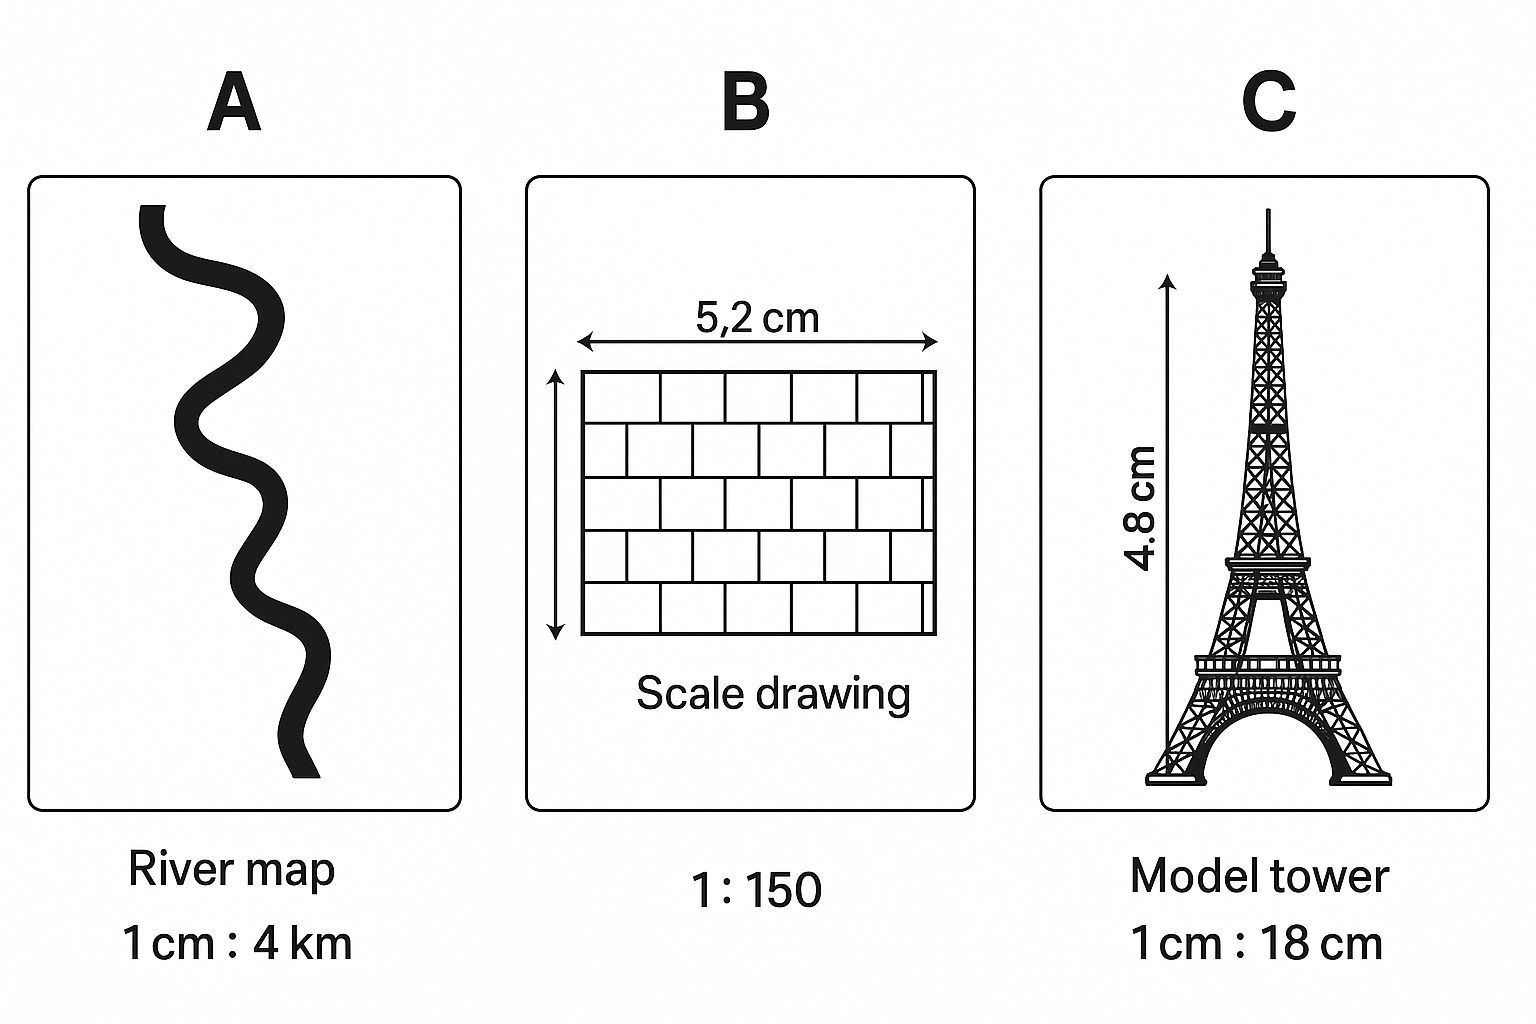
\includegraphics[width=0.94\linewidth,height=0.49\textheight,keepaspectratio]{web-diagrams/excellence-composite-2.png}
\end{center}
\vspace{0.35em}
\noindent\begin{minipage}[t]{0.275\linewidth}\vspace{0pt}\textbf{4.} Use the river map to estimate the real river length and explain whether $12$ km is reasonable.\end{minipage}\hspace{0.08\linewidth}\begin{minipage}[t]{0.275\linewidth}\vspace{0pt}\textbf{5.} Use the patio drawing to estimate the real dimensions in metres.\end{minipage}\hspace{0.08\linewidth}\begin{minipage}[t]{0.275\linewidth}\vspace{0pt}\textbf{6.} Use the tower measurements to estimate the real tower height and round to the nearest cm.\end{minipage}\par

\vspace{1.0em}
\noindent\begin{minipage}[t]{0.46\linewidth}\vspace{0pt}\textbf{7.} A student says a gate drawn as $1.6$ cm on a $1:200$ scale must be $1.6$ m wide. Explain the mistake and give a better estimate.\end{minipage}\hfill\begin{minipage}[t]{0.46\linewidth}\vspace{0pt}\textbf{8.} A photo scale is $1$ cm : $30$ cm. An object is $6.1$ cm tall in the photo. Estimate the real height and state it in metres.\end{minipage}
\end{document}
